\documentclass[../main.tex]{subfiles}

\makeatletter
\@ifundefined{fromRoot}{%
  \newcommand{\fromRoot}[1]{../#1}
  
  \usepackage{xr}
  \externaldocument{../main}
}{}

\def\input@path{{\subfix{../}}}
%or: \def\input@path{{/path/to/folder/}{/path/to/other/folder/}}
\makeatother

\graphicspath{{\subfix{../}}}

\hypersetup{
    pdfauthor   = {Camille MONIÈRE},
    pdftitle    = {Th\`{e}se (Présentation: contexte)},
    pdfsubject  = {Th\`{e}se (Présentation: contexte)},
%    pdfkeywords = {mots-cl\'{e}s},
}

\begin{document}

\section{Introduction}

\subsection{Contexte}

\begin{frame}{Télécommunications numériques sans-fil}
  \begin{columns}
    \begin{column}{.4\linewidth}
      \begin{center}
        \placeholder{width=.85\linewidth, height=.6\textheight}
        \captionof{figure}{Illustration : une antenne, deux devices.}
      \end{center}
    \end{column}
    \begin{column}{.6\linewidth}
      \small
      \begin{overlayarea}{\linewidth}{.55\textheight}
        \begin{ctrlitemize}{1em}
          \item Plus fiables et résilients que leurs pendants analogiques.
          \item<2-> Champ regroupant :
          \begin{ctrlitemize}{1ex}
            \scriptsize
            \item<2-> les réseaux cellulaires \\\hspace{1em} \textit{3G, 4G/LTE, 5G},
            \item<3-> les réseaux en champs proches \\\hspace{1em} \textit{ZigBee, NFC, Bluetooth},
            \only<4>{\item et les réseaux longues portées basses puissances \acrshortpl{lpwan} \\\hspace{1em} \textit{LoRa/LoRaWAN, SigFox, NB-IoT}.}
            \only<5->{\item et \textbf{\textcolor{red}{les réseaux longues portées basses puissances \acrshortpl{lpwan}}} \\\hspace{1em} \textit{LoRa/LoRaWAN, SigFox, NB-IoT}.}
          \end{ctrlitemize}
        \end{ctrlitemize}
      \end{overlayarea}
    \end{column}
  \end{columns}
\end{frame}

\begin{frame}{\acrfullpl{lpwan}}
  \begin{overlayarea}{\linewidth}{.2\textheight}
  Les \acrshortpl{lpwan} ont connu un fort développement durant la dernière décennie, de nombreux standards ont vu le jour \footnotemark.
  \end{overlayarea}

  \begin{overlayarea}{\linewidth}{.6\textheight}
    \only<1>{
      \begin{columns}
        \begin{column}{.3\linewidth}
          \hfill
        \end{column}
        \begin{column}{.6\linewidth} \centering
          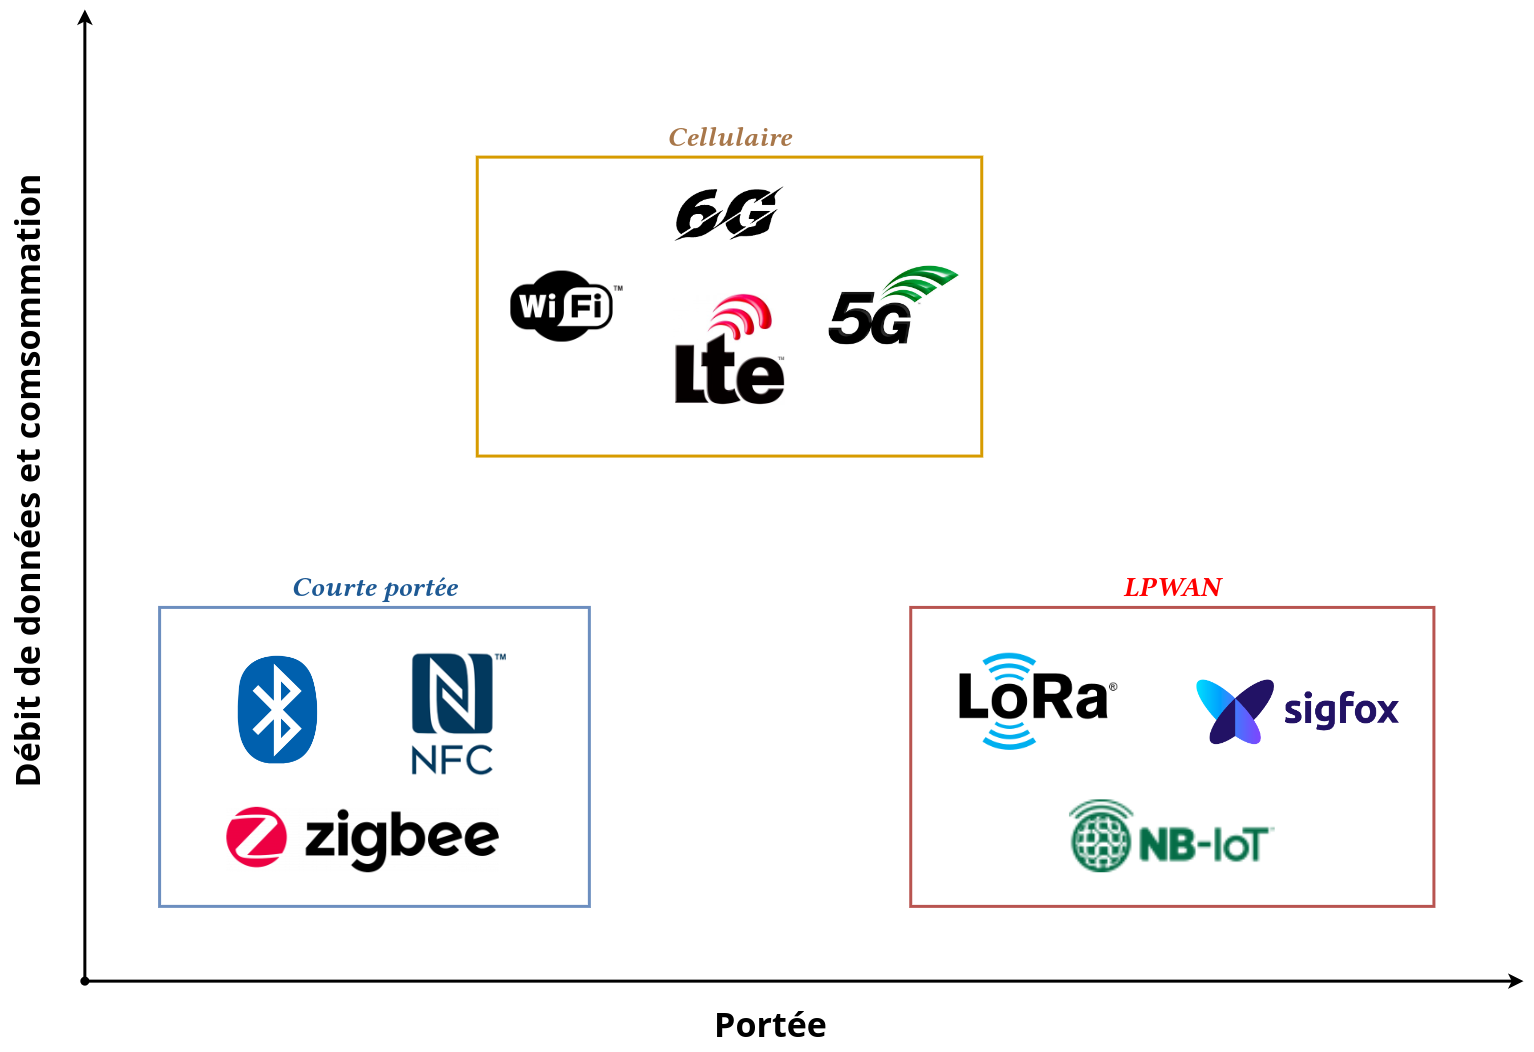
\includegraphics[width=\linewidth]{figures/drawiopdf/lpwan_and_co}
        \end{column}
        \begin{column}{.1\linewidth}
          \hfill
        \end{column}
      \end{columns}
    }
    \only<2>{
      \begin{center}
        % \newcommand{\coltab}[2]{%
        %   \begingroup
        %   \ra{1.}
        %   \begin{tabular}{@{}#1@{}}
        %     #2
        %   \end{tabular}
        %   \endgroup
        % }%
        \ra{1.2}
        % \centering
        % \label{chapter:sota:tab:lpwan-tech}
        % \begin{noindent}
          \scriptsize
          \begin{tabular}{@{}r@{\phantom{XXX}}r@{\phantom{XX}}r@{\phantom{XX}}r@{}}
            \toprule
                                   & \textbf{SigFox}   & \textbf{LoRa}     & \textbf{NB-IoT} \\ \midrule
            \textbf{Modulation}    & \acrshort{bpsk}   & \acrshort{css}    & \acrshort{qpsk} \\ 
            \textbf{Central frequency}
                                   & $868$ MHz         & $868$ MHz         & LTE Bands       \\
            \textbf{Bandwidth}     & $0.1$ kHz         & $125$/$250$ kHz   & $200$ kHz       \\
            \textbf{Max data rate} & $0.1$ kb/s        & $50$ kb/s         & $200$ kb/s      \\
            \textbf{Max payload length}
                                   & $96$ bits         & $1944$ bits       & $12.8$ kilobits \\
            \textbf{Urban range}   & $10$ km           & $5$ km            & $1$ km          \\
            \textbf{Rural range}   & $40$ km           & $20$ km           & $10$ km         \\
            \textbf{Interference resilience}
                                   & very high         & very high         & low             \\
            \textbf{Error correcting code}
                                   & none              & Hamming codes     & Conventional codes \\
            \bottomrule
          \end{tabular}
          % \end{noindent}
        \captionof{table}{Overview of the features offered by three \acrshort{lpwan} technologies, SigFox, LoRa and NB-IoT.}
        \ra{1}
      \end{center}
    }
  \end{overlayarea}
  \footnotetext{\cite{goursaudDedicatedNetworksIoT2015, sinhaSurveyLPWATechnology2017}}
\end{frame}


\begin{frame}{Problème des préambules}
  \textbf{TODO, 1 ou 2 slides}
\end{frame}


\subsection[Le projet \acrshort{qcsp}]{Le projet \acrfull{qcsp}}

\begin{frame}{\subsecname}{}
  \begin{center}
    
\includegraphics[width=0.6\linewidth]{figures/logos-thesis/partners-logos.png}
  \end{center}
\end{frame}

\begin{frame}{Principes de \acrshort{qcsp}}
  \textbf{TODO, le spatial, le ccsk et le nbldpc}
\end{frame}

\begin{frame}{\acrfull{ccsk}}
  \textbf{TODO, animation comment on module et comment on démodule}
\end{frame}

\begin{frame}{\acrfull{ldpc}}
  \textbf{TODO, TRES SUCCINCT, vitye fait trois VN et un CN, pour completion}
\end{frame}


\end{document}
